\documentclass{izvjestaj}

\usepackage{amsmath}
\usepackage{amssymb}
\usepackage{amsfonts}
\usepackage{theorem}
\usepackage{array}
\usepackage{subfigure}
\usepackage{graphicx}
\usepackage[small,bf]{caption}
\usepackage{enumerate}
\renewcommand{\labelitemi}{$-$}


\vjezba{Naziv vježbe}
\prezime{Prezime}
\ime{Ime}
\jmbag{JMBAG}
\grupa{XY}			% grupa laboratorijske vježbe
\profil{Profil}
\predmet{Naziv kolegija}
\datum{Datum}
\broj{XX}			% redni broj vježbe


\begin{document}


\maketitle

\section{Opis vježbe}

Izvještaj sa laboratorijskih vježbi piše se jasno, ne previše opširno ali ne i previše sažeto, prema strukturi korištenoj u ovome dokumentu. Prilikom pisanja izvještaja koristi se bezlični književni jezik, a potrebno je paziti na pravopis. 

Tekst je potrebno poravnati obostrano, a slike i tablice centrirano. Svaka slika i tablica mora imati sažeti naslov koji se nalazi iznad tablice, odnosno ispod slike. Tablice moraju biti jednostavne, lako čitljive i razumljive.

Opis vježbe sadrži opis eksperimenta i opis laboratorijskog modela te se svaki dio piše u 5 do 10 rečenica. Uz to, obvezno je navesti podatke korištene opreme. Podatci se daju tablično, a nalaze se na natpisnoj pločici i zovu se nazivni podaci, a ne karakteristike. Nazivne podatke je potrebno ispravno prepisati s natpisne pločice, a ako je stroj rađen za američko i europsko tržište, prepisuju se samo podaci za europsko tržište.

\section{Odzivi}

Primjer dobrog prikaza odziva dan je slikom  \ref{fig:slika}, a preporuča se korištenje nekog od dostupnih alata za crtanje odziva.

	\begin{figure}[!htb]
	\centering
	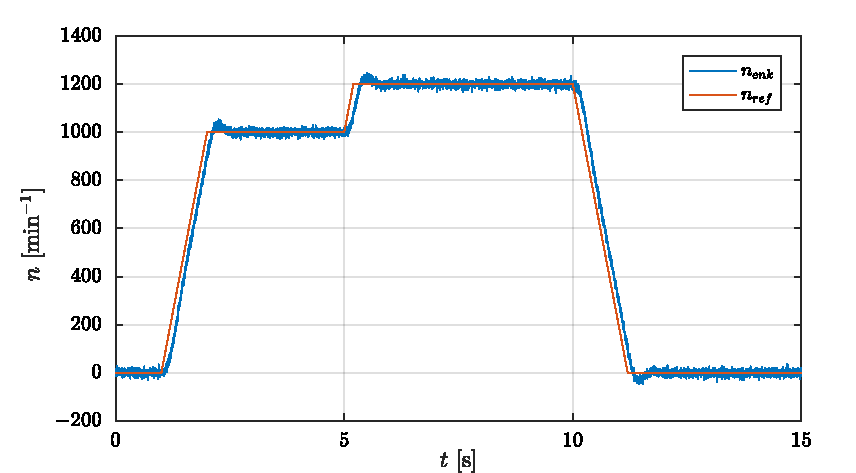
\includegraphics{slika.pdf}
	\caption{Odziv brzine vrtnje}
	\label{fig:slika}
	\end{figure} 

Prilikom izrade slika potrebno je obratiti pažnju na:

\begin{itemize}
\item Osi grafova moraju biti označene i na njima trebaju biti navedene mjerne jedinice.
\item Vrijeme ne može biti negativno što se događa kada koristite \emph{pretrigger} opciju. Predlaže se korištenje \emph{pretrigger} opcije i pomicanje vektora vremena za iznos \emph{pretrigger} vremena.
\item Vremenska skala uobičajeno se daje u sekundama. Predlaže se ispravno skaliranje vektora vremena.
\item Graf treba optimalno iskoristiti tako da bude što manje bijelog prostora. Predlaže se ispravno podešavanje najmanje i najveće vrijednost na osima grafa tako da se prikazuje samo onaj dio krivulje koji se analizira.
\item Svaki graf mora imati pomoćnu koordinatnu mrežu (\emph{grid} opcija).
\item Na jednom grafu prikazuju se samo one veličine koje imaju istu mjernu jedinicu. U slučaju da graf prikazuje dvije ili više veličina potrebno je svaku od njih crtati drugačijom bojom, a u legendi grafa označiti koja je veličina prikazana kojom bojom.
\item Koriste se umjerene i vidljive boje, a nije potrebno svaki graf crtati drugačijom bojom.
\end{itemize}

Također, prilikom unosa slike u izvještaj potrebno je paziti da se unese cijela slika tako podaci i skale budu vidljivi.


\section{Komentari odziva}

U ovom se poglavlju komentiraju odzivi prikazani u prethodnom poglavlju. Komentira se svaka radna točka, promjena radne točke i svaka prikazana veličina. 

\section{Zaključak}

Izvještaj mora sadržavati zaključak. Izraženi zaključak mora biti opsežniji od tvrdnje da se eksperimentalni rezultati poklapaju sa teoretskim pretpostavkama.

\end{document}